%!TEX root = ../main-anran-ma.tex 
% so I can build in this tex file too. 
%************************************************
\chapter{Background}\label{ch:background}
%************************************************
\renewcommand{\thefigure}{\arabic{chapter}.\arabic{figure}}
\renewcommand{\thetable}{\arabic{chapter}.\arabic{table}}

\paragraph{Motivation}
In 1739, the Scottish philosopher David Hume questioned why we know that the sun will rise tomorrow, ``\textit{tho' 'tis plain we have no further assurance of these facts, than what experience affords us}''~\cite{hume1896}. 
Hume's question about causality is daunting, yet most of us are not in crisis because we doubt if the sun rises tomorrow. 
The reason is probably that we believe in physics, astrology, and the rules and formulas that assure us the universe works in a certain way, hence the sun rises tomorrow. 
It is exactly the rules and formulas this thesis attempts to investigate, in the realm of computer programs, with which we are certain that the equivalent version of the sun in a program will rise tomorrow. 

Computer programs are ubiquitous in almost every aspect of human life. 
We want them to solve our problems efficiently, and correctly. 
Fortunately, brilliant scientists and engineers have taken the matter into their hands. 
A recent example is seL4~\cite{klein09}, the first formally proven operating system kernel against overflows, memory leaks, non-termination, etc. using the interactive theorem prover Isabelle/HOL~\cite{nipkow2002isabelle}. 
Its verification brings great potential to safety-critical fields like aircrafts and autonomous cars, the latter of which is to be in mass production in 2024.\footnote{\url{https://sel4.systems/news/2023\#nio-skyos}, accessed 2024.03.10. }

Imagine soon being driven by an autonomous car carrying seL4. 
It is desirable that it delivers us to the correct destination, and never get stuck driving around the same block without making progress. 
Delivering the correct result and stopping eventually is called \define{total correctness}. 
% Once we know that a program is totally correct, then we are sure that the sun rises tomorrow. 

To know ``for sure'', we could verify programs using formal methods. 
One famous method is \define{Hoare triples}~\cite{hoare69}. 
A Hoare triple contains three parts: a precondition, a program, and a postcondition. 
They are written as such: \hoare{G}{C}{F}.
%%\footnote{Originally it was written as $F \{C\} G$, but now it is often written with brackets around conditions instead of the program.} 
It states that if the system starts in a state that satisfies the precondition, then the state after the execution of the program will satisfy the postcondition, provided that the program terminates.
Hoare triples are elegant in that once we have appropriate preconditions, we can follow their reference rules on sequential programs with ease. 
With Hoare triples in their original form, we know the program is correct, but we are not sure of its termination. 
This is called \define{partial correctness}. 

To prove a program totally correct, Dijkstra presented the \define{weakest precondition transformer}~\cite{dijkstra75} (wp): starting with a postcondition, it works backwards and calculates what the weakest precondition is that guarantees both correctness and termination. 
A predicate $P$ is considered to be \define{weaker} than $Q$, if $Q\implies P$ is valid. 
Conversely, $Q$ is \define{stronger} than $P$. 
In Hoare triples, the precondition is a \imptt{sufficient} condition for the program to be correct in that the final state will satisfy the desired postcondition, while with wp we obtain a \imptt{necessary and sufficient} precondition. 
Relaxing the commitment for termination, Dijkstra also proposed the \define{weakest liberal precondition transformer}~\cite{dijkstra90} (wlp) which delivers preconditions so that the program either terminates correctly or never terminates, proving partial correctness. 
The name contains the word \define{liberal}, in the sense that the wlp transformer takes a more ``liberal'' view on non-termination: divergence or execution forever is considered as acceptable in this case. 

Since then, a plethora of research projects blossomed and yielded fruitful results. 
Not only did Hoare Logic receive numerous copious attention during the first decade of its proposal~\cite{apt81}, it has become the basis for program verification now~\cite{gordon2010ForwardHoare}. 
Hoare triple also finds applications in low-level programming languages~\cite{myreen07}, quantum programs~\cite{zhou19}, distributed real-time systems~\cite{hooman1994extending}, and so on. 

Likewise, Dijkstra's wp transformer also spawned various scientific work on probabilistic programs~\cite{kaminski2016weakest}, quantum programs~\cite{boreale20}, continuous programs~\cite{liu22}, and so much more.
Especially inspiring for this thesis is the work by O'Hearn named \define{incorrectness logic}~\cite{ohearn2020IncorrectnessLogic}. 
It studies an underapproximation (subset) of the \define{strongest postcondition transformer}~\cite{dijkstra90} (sp) by Dijkstra, focusing on reachability of final states to prove the existence of bugs. 
He proposed the incorrectness triple starting from the implication 
$$F\implies sp.C.G$$
Here, $F$ is an underapproximation of the strongest postcondition of precondition $G$ w.r.t. program $C$, whereas in this thesis, we attempt to study the implication 
$$wlp.C.F\implies G$$ 
where $G$ is an overapproximation of the strongest liberal precondition of postcondition $F$ w.r.t program $C$. 
Despite focusing on different transformers and relations, incorrectness logic gives great intuition on how to approach the overapproximation over wlp.

\paragraph{Contribution}
This thesis yields results regarding in pre- and postcondition transformers and the implication $wlp.C.F\implies G$. 
The results are listed below in chronological order: 
\begin{enumerate}
    \item We prove that the definition of the weakest precondition transformer of while-programs by Dijkstra~\cite{dijkstra75} and the one using the least fixed point coincide, and give intuition to explain the necessity of using the least fixed point instead of using any other fixed point. 
    \item Following the previous result, we deduce that the greatest fixed point is necessary to define the weakest liberal precondition. 
    \item We relate the pre- and postcondition transformers under angelic or demonic considerations over non-determinism using relations like termination, reachability, conjugation, implication, and equivalence. 
    We then show the results as a graph in \autoref{fig:wp-sp-relation}.
    % \begin{figure}[!h]
    %     \centering
    %     \includesvg[width=.9\linewidth]{image/wp-sp-relation-h.svg}
    %     \caption{Relating wp, wlp, sp, slp}
    %     \label{fig:intro-wp-sp-galois}
    % \end{figure}
    \item We discuss all possible scenarios of the overapproximation $wlp.C.F\implies G$, what we call the \define{necessary liberal preconditions}, concluding that without further restrictions, the overapproximate $G$ can contain any initial states. However, we show that the only certainty is that initial states satisfying $\neg G$ will lead to termination in states satisfying $\neg F$. Following this, we demonstrate the usefulness of this overapproximation with an example. 
    \item We also provide a proof system that captures this overapproximation triple, and prove its soundness. 
    \item We also notice a special group of initial states, starting from which the execution is possible to terminate satisfying both the desired postcondition and its opposite, like the green parts in \autoref{fig:intro-g}. 
    \begin{figure}[t]
        \centering
        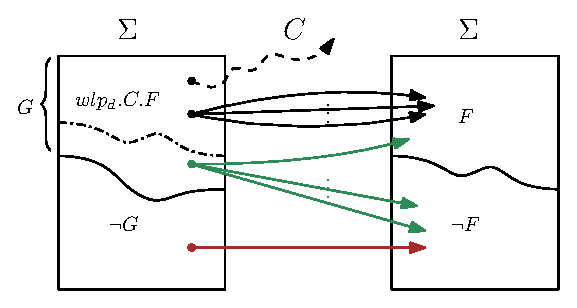
\includegraphics[width=.6\linewidth]{image/wlp-g/wlp-g-gg.eps}
        \caption{Necessary Liberal Precondition $G$ That Additionally Has Green Dots}
        \label{fig:intro-g}
    \end{figure}
    We capture these preconditions by approaching from top and bottom, namely finding scenarios in which the necessary liberal precondition $G$ underapproximates these special preconditions, and finding scenarios where $G$ overapproximates them. In this way, we can establish an equivalence between $G$ and wlp added with the special preconditions, given constraints. This $G$ is exactly wlp with angelic non-determinism. 
    \item We discover a type of preconditions that we name $wp_d^+$. They serve as the ``cut'' between partial correctness and partial incorrectness, in the sense that $wp_d^+.C.F$ corresponds to partial correctness, and $\neg wp_d^+.C.F$ corresponds to partial incorrectness. 
\end{enumerate}


\paragraph{Outline}
After explaining our motivation in this chapter, we proceed to build the formal foundations of the formalism used in this thesis in \autoref{ch:Preliminaries}. 
We first present a table of notations we adopt, then give a soft introduction of Hoare logic in \autoref{sec:hoare}, followed by Dijkstra's \define{Guarded Command Language}, which we use throughout the thesis. 
Then we display the weakest precondition transformer in \autoref{sec:wp}, comparing it against Hoare logic, then give a detailed discussion about the use of fixed points while defining while loops. 
Finally, we add the notion of non-determinism to the wp transformer, and discuss the difference between angelic and demonic non-determinism and explain our design choice. 

Following this, we show the weakest liberal precondition transformer in \autoref{sec:wlp} and the strongest postcondition transformer in \autoref{sec:sp}. 
Subsequently, we introduce a \define{big-step semantics} in \autoref{sec:big-step}  and \define{collecting semantics} in \autoref{sec:collecting} to help us reason about the semantics of the aforementioned transformers in \autoref{sec:sound} and list some properties in \autoref{sec:prop}.

In \autoref{ch:appr}, we first relate wp, wlp, sp, and slp together using various relations, then illustrate them in a graph. 
This helps us distinguish the necessary liberal precondition with other implications that are researched, so that we can analyze the scenarios of our overapproximation in \autoref{ch:nlp}. 
Then we provide examples to convey the usefulness of this overapproximation, and show its proof system as well as prove its soundness. 
We then discover a special scenario that is of interest, and find restraints that qualify this special scenario, then prove their correctness in \autoref{sec:special}. 
We also show the class of predicate transformer we call $wp_d^+$, which serves as the ``cut'' between partial correctness and partial incorrectness. 
Finally, we summarize our conclusions in \autoref{ch:conclusion} and propose possible future work. 






% wp is concerned with total correctness and is related to Hoare triples by an implication: 
% \footnote{Here $wp.C.F$ is a function written in lambda-calculus style, it can be seen now as a function $wp(C,F)$. This form of writing proves to be simple and elegant in the upcoming sections.}
% \[\forall G.\ G\implies wp.C.F: \{G\} C \{F\}\]
% This connection not only tells us that 
% \begin{itemize}
%     \item[-] given $wp.C.F$, any predicate $G$ that implies it can be the precondition of a valid Hoare Triple: $\{G\} C \{F\}$; 
% \end{itemize}
% it also shows when Hoare Triple will guarantee total correctness: 
% \begin{itemize}
%     \item[-] given a valid Hoare Triple $\{G\} C \{F\}$, if its precondition $G$ implies $wp.C.F$, then $\{G\} C \{F\}$ is valid for total correctness. 
% \end{itemize}

% Sometimes, however, we deem nontermination a good behaviour, and proving partial correctness suffices. 
% The \define{weakest liberal precondition} transformer \cite{Dijkstra90} can be used in such occasions: 
% if the system is in a state satisfying $wlp.C.F$, then either $F$ is reachable after the termination of $C$, or $C$ does not terminate.
% wlp directly relates to Hoare triples via an implication: 
% \[\forall G.\ G\implies wlp.C.F: \{G\} C \{F\}\]
% $G$ is then called the \define{sufficient liberal precondition}, and finding it means we can prove the absense of errors in the program (if it terminates). 
% In contrast, the \define{necessary liberal precondition} $G$ (where $ wlp.C.F\implies G$) tells us that the system will not satisfy the postcondition $F$, once $G$ is violated. 
% Cousot et al. studied the matter from a practical perspective~\cite{Cousot13}, they proposed inference tools and experimented in industrial codes.
% In this thesis, we aim to research this matter further with a more theoretical view. 
% We would like to propose a proof system and prove its soundness and completeness similar as in \cite{Vries11}, but using Dijkstra's guarded command language (GCL)~\cite{Dijkstra75}. 

% Instead of the usual qualitative reasoning using logical predicates, we would like to study in a quantitive setting using functions that represent quantities such as expectations of program variables. 
% While predicates map program states to true or false, functions map program states to $R\infty$, real numbers extended with (negative) infinity. 
% In this setting, not only are infinities clear indication for nontermination, the transformers can also express more such as flow of quantitive information~\cite{Zhang22}.

